\documentclass[runningheads]{../../../llncs}
\usepackage[paperheight=295mm,paperwidth=210mm]{geometry}
\usepackage{graphicx}
\usepackage{import}
\usepackage{kotex}
\usepackage[dvipsnames]{xcolor}
\usepackage{fancyvrb}
\usepackage{listings}
\usepackage{indentfirst}
\usepackage{tabularx}
\usepackage{underscore}
\usepackage{multicol}
\usepackage{enumitem}
\usepackage{menukeys}
\usepackage{amsmath}
\usepackage{clrscode3e} % https://www.ctan.org/pkg/clrscode3e?lang=en
\usepackage[numbers,square,super]{natbib}
\usepackage{inconsolata} % Inconsolata
\usepackage{mathptmx} % Times New Roman
\usepackage{minted}
\graphicspath{ {./images/} }
\lstset{basicstyle=\footnotesize\ttfamily,breaklines=true}
\renewcommand{\bibname}{참고문헌}
\setlength{\parindent}{1em}
\setlength{\parskip}{1em}
\linespread{1.2}
{\renewcommand{\arraystretch}{1.5}%
\setlength{\tabcolsep}{0.5em}%
\newenvironment{Figure}
  {\par\medskip\noindent\minipage{\linewidth}}
  {\endminipage\par\medskip}
\newcommand{\translation}[1]{\textsuperscript{#1}}
\newlist{algorithm}{enumerate}{10}
\setlist[algorithm]{label*=\arabic*.}
\setlist[algorithm,1]{label=\textbf{\arabic*}}
\setlist[algorithm,2]{label=\textbf{\alph*}}
\setlist[algorithm,3]{label=\textbf{\roman*}}
\setlist[algorithm,4]{label=(\arabic*)}
\setlist[algorithm,5]{label=(\alph*)}
\setlist[algorithm,6]{label=(\roman*)}
\makeatletter
\renewcommand\NAT@citesuper[3]{\ifNAT@swa
\if*#2*\else#2\NAT@spacechar\fi
\unskip\kern\p@\textsuperscript{\NAT@@open#1\if*#3*\else,\NAT@spacechar#3\fi\NAT@@close}%
   \else #1\fi\endgroup}
\makeatother
	
\begin{document}

\title{CSE3013 (컴퓨터공학 설계 및 실험 I) \space \newline PRJ-1 테트리스 프로젝트 1주차 예비 보고서}
\author{서강대학교 컴퓨터공학과 박수현 (20181634)}
\institute{서강대학교 컴퓨터공학과}
\maketitle

\section{목적}
테트리스의 구조와 테트리스를 구성하는 각 함수의 기능을 이해한다.

\newpage

\section{문제}
\subsection{테트리스 순서도}

\tikzset{every picture/.style={line width=0.75pt}} %set default line width to 0.75pt      
% Generated by https://www.mathcha.io/editor#
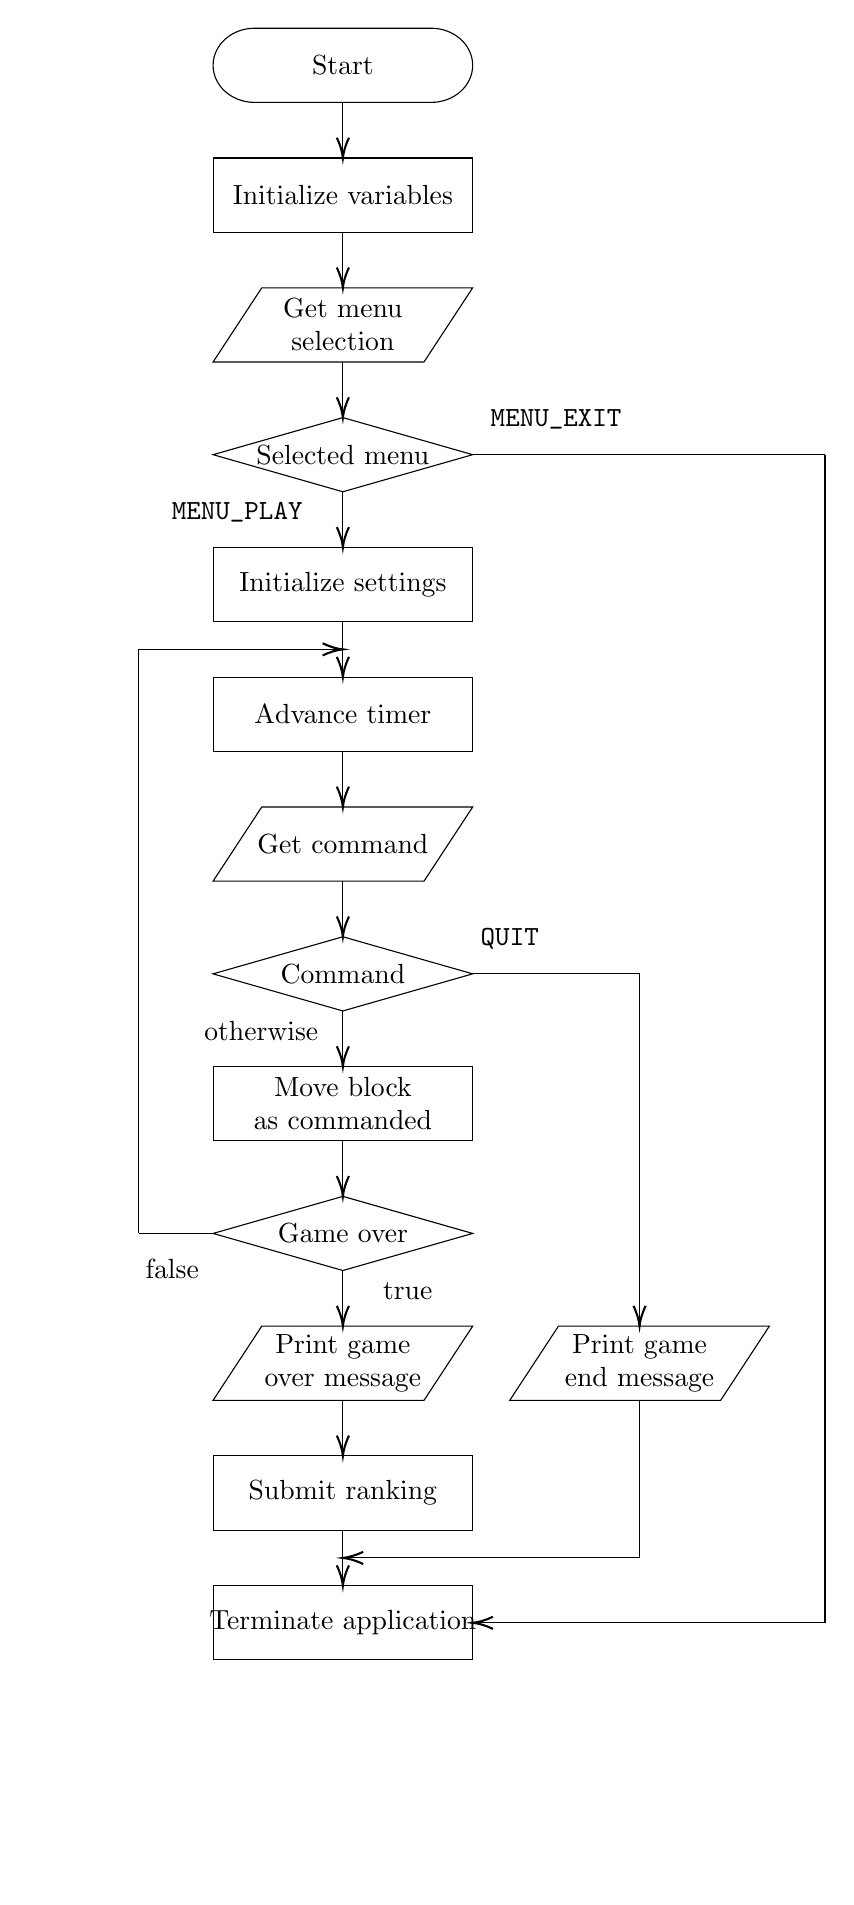
\begin{tikzpicture}[x=0.67pt,y=0.67pt,yscale=-1,xscale=1]
\path (100,1027); %set diagram left start at 0, and has height of 1027  

\draw   (222.4,30) -- (317.6,30) .. controls (329.97,30) and (340,38.95) .. (340,50) .. controls (340,61.05) and (329.97,70) .. (317.6,70) -- (222.4,70) .. controls (210.03,70) and (200,61.05) .. (200,50) .. controls (200,38.95) and (210.03,30) .. (222.4,30) -- cycle ;
\draw   (200,100) -- (340,100) -- (340,140) -- (200,140) -- cycle ;
\draw    (270,70) -- (270,98) ;
\draw [shift={(270,100)}, rotate = 270] [color={rgb, 255:red, 0; green, 0; blue, 0 }  ][line width=0.75]    (10.93,-3.29) .. controls (6.95,-1.4) and (3.31,-0.3) .. (0,0) .. controls (3.31,0.3) and (6.95,1.4) .. (10.93,3.29)   ;
\draw   (226.25,170) -- (340,170) -- (313.75,210) -- (200,210) -- cycle ;
\draw    (270,140) -- (270,168) ;
\draw [shift={(270,170)}, rotate = 270] [color={rgb, 255:red, 0; green, 0; blue, 0 }  ][line width=0.75]    (10.93,-3.29) .. controls (6.95,-1.4) and (3.31,-0.3) .. (0,0) .. controls (3.31,0.3) and (6.95,1.4) .. (10.93,3.29)   ;
\draw   (270,520) -- (340,540) -- (270,560) -- (200,540) -- cycle ;
\draw    (270,210) -- (270,238) ;
\draw [shift={(270,240)}, rotate = 270] [color={rgb, 255:red, 0; green, 0; blue, 0 }  ][line width=0.75]    (10.93,-3.29) .. controls (6.95,-1.4) and (3.31,-0.3) .. (0,0) .. controls (3.31,0.3) and (6.95,1.4) .. (10.93,3.29)   ;
\draw   (200,310) -- (340,310) -- (340,350) -- (200,350) -- cycle ;
\draw    (270,280) -- (270,308) ;
\draw [shift={(270,310)}, rotate = 270] [color={rgb, 255:red, 0; green, 0; blue, 0 }  ][line width=0.75]    (10.93,-3.29) .. controls (6.95,-1.4) and (3.31,-0.3) .. (0,0) .. controls (3.31,0.3) and (6.95,1.4) .. (10.93,3.29)   ;
\draw   (200,590) -- (340,590) -- (340,630) -- (200,630) -- cycle ;
\draw   (226.25,730) -- (340,730) -- (313.75,770) -- (200,770) -- cycle ;
\draw   (270,240) -- (340,260) -- (270,280) -- (200,260) -- cycle ;
\draw    (270,560) -- (270,588) ;
\draw [shift={(270,590)}, rotate = 270] [color={rgb, 255:red, 0; green, 0; blue, 0 }  ][line width=0.75]    (10.93,-3.29) .. controls (6.95,-1.4) and (3.31,-0.3) .. (0,0) .. controls (3.31,0.3) and (6.95,1.4) .. (10.93,3.29)   ;
\draw   (200,380) -- (340,380) -- (340,420) -- (200,420) -- cycle ;
\draw   (270,660) -- (340,680) -- (270,700) -- (200,680) -- cycle ;
\draw   (200,800) -- (340,800) -- (340,840) -- (200,840) -- cycle ;
\draw   (226.25,450) -- (340,450) -- (313.75,490) -- (200,490) -- cycle ;
\draw   (200,870) -- (340,870) -- (340,910) -- (200,910) -- cycle ;
\draw    (270,350) -- (270,378) ;
\draw [shift={(270,380)}, rotate = 270] [color={rgb, 255:red, 0; green, 0; blue, 0 }  ][line width=0.75]    (10.93,-3.29) .. controls (6.95,-1.4) and (3.31,-0.3) .. (0,0) .. controls (3.31,0.3) and (6.95,1.4) .. (10.93,3.29)   ;
\draw    (270,420) -- (270,448) ;
\draw [shift={(270,450)}, rotate = 270] [color={rgb, 255:red, 0; green, 0; blue, 0 }  ][line width=0.75]    (10.93,-3.29) .. controls (6.95,-1.4) and (3.31,-0.3) .. (0,0) .. controls (3.31,0.3) and (6.95,1.4) .. (10.93,3.29)   ;
\draw    (270,490) -- (270,518) ;
\draw [shift={(270,520)}, rotate = 270] [color={rgb, 255:red, 0; green, 0; blue, 0 }  ][line width=0.75]    (10.93,-3.29) .. controls (6.95,-1.4) and (3.31,-0.3) .. (0,0) .. controls (3.31,0.3) and (6.95,1.4) .. (10.93,3.29)   ;
\draw    (270,630) -- (270,658) ;
\draw [shift={(270,660)}, rotate = 270] [color={rgb, 255:red, 0; green, 0; blue, 0 }  ][line width=0.75]    (10.93,-3.29) .. controls (6.95,-1.4) and (3.31,-0.3) .. (0,0) .. controls (3.31,0.3) and (6.95,1.4) .. (10.93,3.29)   ;
\draw    (270,700) -- (270,728) ;
\draw [shift={(270,730)}, rotate = 270] [color={rgb, 255:red, 0; green, 0; blue, 0 }  ][line width=0.75]    (10.93,-3.29) .. controls (6.95,-1.4) and (3.31,-0.3) .. (0,0) .. controls (3.31,0.3) and (6.95,1.4) .. (10.93,3.29)   ;
\draw    (270,770) -- (270,798) ;
\draw [shift={(270,800)}, rotate = 270] [color={rgb, 255:red, 0; green, 0; blue, 0 }  ][line width=0.75]    (10.93,-3.29) .. controls (6.95,-1.4) and (3.31,-0.3) .. (0,0) .. controls (3.31,0.3) and (6.95,1.4) .. (10.93,3.29)   ;
\draw    (270,840) -- (270,868) ;
\draw [shift={(270,870)}, rotate = 270] [color={rgb, 255:red, 0; green, 0; blue, 0 }  ][line width=0.75]    (10.93,-3.29) .. controls (6.95,-1.4) and (3.31,-0.3) .. (0,0) .. controls (3.31,0.3) and (6.95,1.4) .. (10.93,3.29)   ;
\draw    (160,680) -- (200,680) ;
\draw    (160,365) -- (160,680) ;
\draw    (160,365) -- (268,365) ;
\draw [shift={(270,365)}, rotate = 180] [color={rgb, 255:red, 0; green, 0; blue, 0 }  ][line width=0.75]    (10.93,-3.29) .. controls (6.95,-1.4) and (3.31,-0.3) .. (0,0) .. controls (3.31,0.3) and (6.95,1.4) .. (10.93,3.29)   ;
\draw    (340,540) -- (430,540) ;
\draw   (386.25,730) -- (500,730) -- (473.75,770) -- (360,770) -- cycle ;
\draw    (430,540) -- (430,728) ;
\draw [shift={(430,730)}, rotate = 270] [color={rgb, 255:red, 0; green, 0; blue, 0 }  ][line width=0.75]    (10.93,-3.29) .. controls (6.95,-1.4) and (3.31,-0.3) .. (0,0) .. controls (3.31,0.3) and (6.95,1.4) .. (10.93,3.29)   ;
\draw    (430,770) -- (430,855) ;
\draw    (430,855) -- (272,855) ;
\draw [shift={(270,855)}, rotate = 360] [color={rgb, 255:red, 0; green, 0; blue, 0 }  ][line width=0.75]    (10.93,-3.29) .. controls (6.95,-1.4) and (3.31,-0.3) .. (0,0) .. controls (3.31,0.3) and (6.95,1.4) .. (10.93,3.29)   ;
\draw    (340,260) -- (530,260) ;
\draw    (530,260) -- (530,890) ;
\draw    (530,890) -- (342,890) ;
\draw [shift={(340,890)}, rotate = 360] [color={rgb, 255:red, 0; green, 0; blue, 0 }  ][line width=0.75]    (10.93,-3.29) .. controls (6.95,-1.4) and (3.31,-0.3) .. (0,0) .. controls (3.31,0.3) and (6.95,1.4) .. (10.93,3.29)   ;

% Text Node
\draw (270,50) node   [align=center] {Start};
\draw (270,120) node  [align=center] {Initialize variables};
\draw (270,190) node  [align=center] {Get menu\\selection};
\draw (270,540) node  [align=center] {Command};
\draw (270,330) node  [align=center] {Initialize settings};
\draw (213,291) node  [align=center] {\texttt{MENU\_PLAY}};
\draw (270,610) node  [align=center] {Move block\\as commanded};
\draw (270,750) node  [align=center] {Print game\\over message};
\draw (270,260) node  [align=center] {Selected menu};
\draw (226,571) node  [align=center] {otherwise};
\draw (270,400) node  [align=center] {Advance timer};
\draw (270,680) node  [align=center] {Game over};
\draw (270,820) node  [align=center] {Submit ranking};
\draw (270,470) node  [align=center] {Get command};
\draw (270,890) node  [align=center] {Terminate application};
\draw (305,711) node  [align=center] {true};
\draw (178,699) node  [align=center] {false};
\draw (360,521) node  [align=center] {\texttt{QUIT}};
\draw (430,750) node  [align=center] {Print game\\end message};
\draw (385,241) node  [align=center] {\texttt{MENU\_EXIT}};

\end{tikzpicture}

\subsection{게임을 구성하는 함수들의 기능}
\begin{itemize}
    \item \mintinline[breaklines]{c++}{void InitTetris()}: 변수들을 초기화한 후 초기 화면을 그리는 메서드를 실행한다.
    \item \mintinline[breaklines]{c++}{void DrawOutline()}: 테트리스 필드, NEXT 슬롯, 점수 인디케이터 등의 테두리를 그린다.
    \item \mintinline[breaklines]{c++}{int GetCommand()}: 사용자의 입력을 받아 명령으로 해석한다.
    가능한 입력은 방향 키 \keys{\arrowkeyup}, \keys{\arrowkeydown},
    \keys{\arrowkeyright}, \keys{\arrowkeyleft}와 \keys{Space}, \keys{Q}이다.
    \item \mintinline[breaklines]{c++}{int ProcessCommand(int command)}: 해석된 명령을 실행한다.
    명령이 \mintinline[breaklines]{c++}{QUIT}이었을 경우 0, 아닐 경우 1을 반환한다.
    \item \mintinline[breaklines]{c++}{void BlockDown(int sig)}: 블럭을 아래로 내린다. 더 이상 내릴 수 없을 경우
    현재 블럭을 필드에 고정시키고 다음 블럭을 사용한다.
    \item \mintinline[breaklines]{c++}{int CheckToMove(char f[HEIGHT][WIDTH], int currentBlock, int blockRotate, int blockY, int blockX)}:
    명령에 따라 블럭을 이동할 수 있는지 판단한다.
    \item \mintinline[breaklines]{c++}{void DrawChange(char f[HEIGHT][WIDTH], int command, int currentBlock, int blockRotate, int blockY, int blockX)}:
    명령에 의해 바뀐 부분만 필드에 업데이트한다.
    \item \mintinline[breaklines]{c++}{void DrawField()}: 테트리스 필드를 그린다.
    \item \mintinline[breaklines]{c++}{void AddBlockToField(char f[HEIGHT][WIDTH], int currentBlock, int blockRotate, int blockY, int blockX)}:
    필드의 주어진 좌표에 현재 블럭을 고정시킨다.
    \item \mintinline[breaklines]{c++}{int DeleteLine(char f[HEIGHT][WIDTH])}: 꽉 찬 줄이 있는지 체크하고, 있을 경우 줄을 지우고 스코어를 증가시킨다.
    \item \mintinline[breaklines]{c++}{void gotoyx(int y, int x)}: 커서를 해당 좌표로 이동시킨다.
    \item \mintinline[breaklines]{c++}{void DrawNextBlock(int *nextBlock)}: NEXT 슬롯에 다음에 나올 블럭 정보를 표시한다.
    \item \mintinline[breaklines]{c++}{void PrintScore(int score)}: 점수를 표시한다.
    \item \mintinline[breaklines]{c++}{void DrawBox(int y, int x, int height, int width)}: 해당 좌표에 특정 크기의 직사각형을 그린다.
    \item \mintinline[breaklines]{c++}{void DrawBlock(int y, int x, int blockID, int blockRotate, char tile)}: 해당 좌표에 특정 모양의 블럭을 그린다.
    \item \mintinline[breaklines]{c++}{void DrawShadow(int y, int x, int blockID, int blockRotate)}: 블럭이 떨어질 위치를 미리 보여 주는 고스트를 그린다.
    \item \mintinline[breaklines]{c++}{void play()}: 게임을 시작한다.
    \item \mintinline[breaklines]{c++}{char menu()}: 메뉴를 그린다.
    \item \mintinline[breaklines]{c++}{void createRankList()}: 랭킹 정보를 구성한다.
    \item \mintinline[breaklines]{c++}{void rank()}: 랭킹 기록들을 그린다.
    \item \mintinline[breaklines]{c++}{void writeRankFile()}: 랭킹이 저장되는 데이터베이스를 생성한다.
    \item \mintinline[breaklines]{c++}{void newRank(int score)}: 새 랭킹 정보를 추가한다.
    \item \mintinline[breaklines]{c++}{int recommend(RecNode *root)}: 추천하는 블럭 배치를 계산한다.
    \item \mintinline[breaklines]{c++}{void recommendedPlay()}: 추천 기능에 따라 블럭을 배치해나가면서 진행되는 게임을 시작한다.
\end{itemize}

\newpage

\subsection{함수 구현}
첫 주에 구현하게 될 함수들에는 다음과 같은 함수들이 있다.

\subsubsection{\proc{CheckToMove}}: 명령에 따라 블럭을 이동할 수 있는지 판단한다.

\begin{codebox}
\Procname{$\proc{CheckToMove}(f, \id{currentBlock}, \id{blockRotate}, \id{blockY}, \id{blockX})$}
\li \For $i \gets 0$ \To $3$
\li \Do
        \For $j \gets 0$ \To $3$
\li     \Do
            \If $\id{block}[i][j] \isequal 1$
\li         \Then
                $x \gets \id{blockX} + j$
\li             $y \gets \id{blockY} + i$
\li             \If $\left( 0 \leq x < \id{WIDTH} \mbox{ and } 0 \leq y < \id{HEIGHT} \right) \neq \const{true}$
\li                 \Then \Return $\const{false}$
                \End
\li             \If $f[y][x] \isequal 1$
\li                 \Then \Return $\const{false}$
                \End
            \End
        \End
    \End
\li \Return $\const{true}$
\end{codebox}

\subsubsection{\proc{DrawChange}}: 명령에 의해 바뀐 부분만 필드에 업데이트한다.

\begin{codebox}
\Procname{$\proc{DrawChange}(f, \id{command}, \id{currentBlock}, \id{blockRotate}, \id{blockY}, \id{blockX})$}
\li \Comment Erase current block
\li \If $\id{command} \isequal \id{KEY\_UP}$
\li \Then $proc{DrawBlock}(blockY, blockX, currentBlock, (blockRotate+3) \mbox{ mod } 4, 0)$ \End
\li \If $\id{command} \isequal \id{KEY\_DOWN}$
\li \Then $proc{DrawBlock}(blockY - 1, blockX, currentBlock, blockRotate, 0)$ \End
\li \If $\id{command} \isequal \id{KEY\_RIGHT}$
\li \Then $proc{DrawBlock}(blockY, blockX - 1, currentBlock, blockRotate, 0)$ \End
\li \If $\id{command} \isequal \id{KEY\_LEFT}$
\li \Then $proc{DrawBlock}(blockY, blockX + 1, currentBlock, blockRotate, 0)$ \End
\li \Comment Draw new block
\li $proc{DrawBlock}(blockY, blockX, currentBlock, blockRotate, 1)$
\end{codebox}

\newpage

\subsubsection{\proc{BlockDown}}: 블럭을 아래로 내린다. 더 이상 내릴 수 없을 경우 현재 블럭을 필드에 고정시키고 다음 블럭을 사용한다.

\begin{codebox}
\Procname{$\proc{BlockDown}(\id{sig})$}
\li \If $\proc{CheckToMove}(f, \id{currentBlock}, \id{blockRotate}, \id{blockY} + 1, \id{blockX})$
\li \Then
        $\id{blockY} = \id{blockY} + 1$
\li     $\proc{DrawChange}(f, \id{command}, \id{currentBlock}, \id{blockRotate}, \id{blockY}, \id{blockX})$
\li \Else
\li     \If $\id{blockY} \isequal 1$
\li     \Then
            $\id{gameOver} \gets \const{true}$
\li     \Else
\li         $\proc{AddBlockToField}(f, \id{currentBlock}, \id{blockRotate}, \id{blockY}, \id{blockX})$
\li         $\id{score} \gets \id{score} + \proc{DeleteLine}(f)$
\li         \Comment Generate new block
\li         $\id{nextBlock}[0] \gets \id{nextBlock}[1]$
\li         $\id{nextBlock}[1] \gets (\mbox{Random integer in 0 .. 6})$
\li         $\id{blockY} \gets -1$, $\id{blockX} \gets (\mbox{Center of field})$
\li         $\proc{DrawField}()$
\li         $\proc{PrintScore}(\id{score})$
        \End
    \End
\end{codebox}

\subsubsection{\proc{AddBlockToField}}: 필드의 주어진 좌표에 현재 블럭을 고정시킨다.

\begin{codebox}
\Procname{$\proc{AddBlockToField}(f, \id{currentBlock}, \id{blockRotate}, \id{blockY}, \id{blockX})$}
\li \For $i \gets 0$ \To $3$
\li \Do
        \For $j \gets 0$ \To $3$
\li     \Do
            \If $\id{block}[i][j] \isequal 1$
\li         \Then
                $f[\id{blockY} + i][\id{blockX} + j] \gets 1$
            \End
        \End
    \End
\li \Return $\const{true}$
\end{codebox}

\newpage

\subsubsection{\proc{DeleteLine}}: 꽉 찬 줄이 있는지 체크하고, 있을 경우 줄을 지우고 스코어를 증가시킨다.

\begin{codebox}
\Procname{$\proc{DeleteLine}(f)$}
\li $erased \gets 0$
\li \For $i \gets 0$ \To $\id{HEIGHT} - 1$
\li \Do
        $flag \gets \const{true}$
\li     \For $j \gets 0$ \To $\id{WIDTH} - 1$
\li     \Do
            \If $f[i][j] \isequal 0$
\li         \Then
                $flag \gets \const{false}$
            \End
        \End
\li     \If $flag \isequal \const{true}$
            \Then
\li             $erased \gets erased + 1$
\li             \For $y \gets i$ \Downto $1$
\li             \Do
                    \For $x \gets 0$ \To $\id{WIDTH} - 1$
\li                 \Do
                        $f[y][x] \gets f[y - 1][x]$
                    \End
                \End
\li             \For $x \gets 0$ \To $\id{WIDTH} - 1$
\li             \Do
                    $f[0][x] \gets 0$
                \End
\li             $i \gets i - 1$
            \End
        \End
    \End
\li \Return $100 \times \id{erased}^2$
\end{codebox}

\end{document}
